\documentclass[../main.tex]{subfiles}
\makeatletter
\@ifundefined{fromRoot}{%
  \newcommand{\fromRoot}[1]{../#1}
  
  \usepackage{xr}
  \externaldocument{../main}
}{}

\def\input@path{{\subfix{../}}}
%or: \def\input@path{{/path/to/folder/}{/path/to/other/folder/}}
\makeatother

\graphicspath{{\subfix{../}}}

\hypersetup{
    pdfauthor   = {Mael Tourres},
    pdftitle    = {Th\`{e}se (Chapitre 2)},
    pdfsubject  = {Th\`{e}se (Chapitre 2)},
%    pdfkeywords = {mots-cl\'{e}s},
}

\begin{document}
\selectlanguage{french}
%
%
%
%
\chapter{Introduction aux codes correcteurs d'erreurs} 
\label{chapter:2}
\chaptermark{Introduction aux codes correcteurs d'erreurs}
%
%
%
%
%
Dans la partie initiale de ce premier chapitre, deux concepts sont introduits : celui de codage canal, une technique avancée utilisée dans les systèmes de communications numériques afin de fiabiliser les transmissions, ainsi que le concept de codes correcteurs d'erreurs (\acrshort{cce}) et leur positionnement dans les chaînes de communications numériques. La seconde partie de ce chapitre présente les principales familles de CCE actuellement utilisées dans différents standards de communication ainsi que les algorithmes de décodage associés communément employés. 
%
%
%
%
%
%
%
\etocsetnexttocdepth{4}
\etocsettocstyle{
    { \large \hspace{-1.5 em} \textbf{} \hfill}
    \vspace{-2.5 em}\\\par\noindent\rule{\linewidth}{1 pt}\vspace{-.2 em}
    }
{\par\noindent\rule{\linewidth}{1 pt}\\}
\localtableofcontents
%
%
%
%
%
%
%
%
\section{Introduction au codage canal}
%
%
%
Durant les deux dernières décennies, la quantité de systèmes communicants présents dans notre environnement a considérablement augmenté. 
Cette évolution rapide a été stimulée par l'émergence de nouveaux standards de communication (3G \cite{3G}, WIFI \cite{wifi}, WiMAX \cite{wimax}, 4G-LTE \cite{Ref_4G}, 5G \cite{5g} et 6G \cite{Ref_6G}), dont le but était de répondre aux nouveaux usages, tout en permettant aux infrastructures de supporter l’augmentation croissante des besoins en termes de bande passante, mais aussi de réduire la consommation énergétique.
Pour atteindre ces objectifs, de nombreux travaux de recherches se sont focalisés sur (a) la proposition de nouvelles formes d'ondes, et (b) la mise au point des algorithmes de traitement du signal associés. 
Ces innovations ont pour vocation de proposer des niveaux de performances élevés (débits, latence, QoS, efficacité énergétique) d’un point de vue théorique, tout en garantissant la faisabilité de ces approches à l’aide de technologies grand public.
%%%%%%%%%%%%%%%%%%%%%%%%%%%%%%%
\begin{figure}[H]
    \centering
    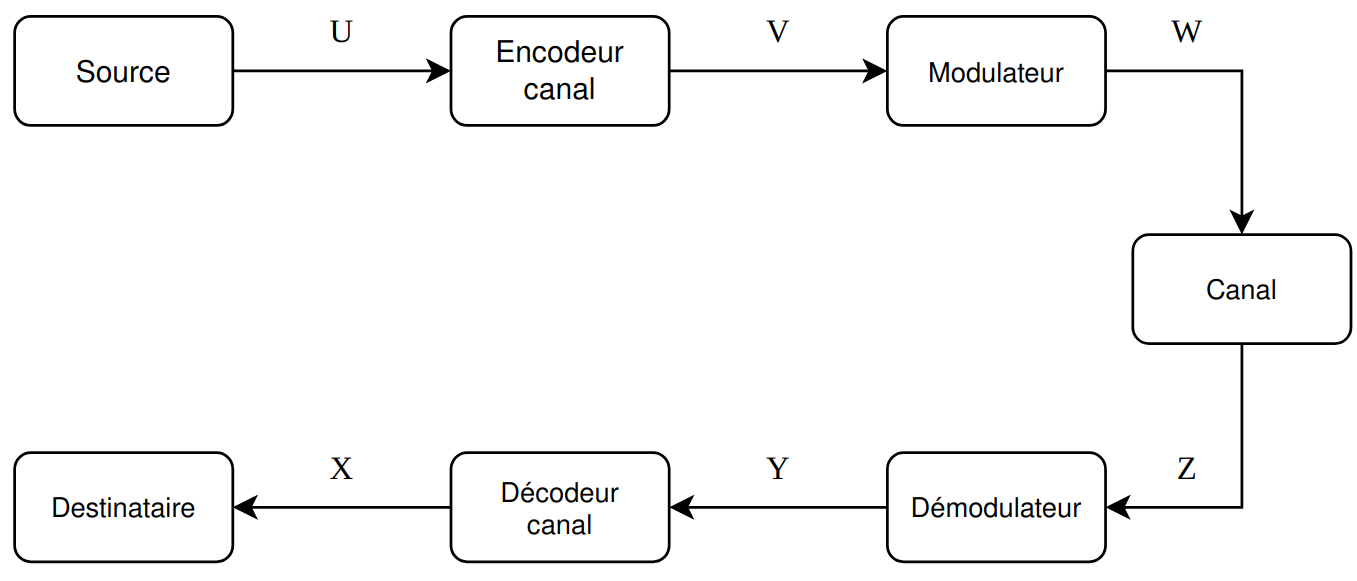
\includegraphics[scale=0.3]{chapter2/figs/chainecom.png}
    \caption{Schéma simplifié d'une chaine de communications numérique}
    \label{chainecom}
\end{figure}
%%%%%%%%%%%%%%%%%%%%%%%%%%%%%%%
Les systèmes de communications numériques visent à permettre la transmission d'informations numériques d'un émetteur (la source) vers un ou plusieurs récepteurs (les destinataires). Ces systèmes peuvent être modélisés de manière simplifiée comme illustré dans la figure \ref{chainecom}, représentant une chaîne de communication numérique.\\
Cette chaîne "gros grain", a été conceptualisée par Claude Shannon en 1948 \cite{Sha48}. Les principales étapes mises en œuvre lors de la transmission de données numériques d'un \textit{émetteur} (source) vers un \textit{récepteur} (destinataire) sont décrites dans ce schéma. L'échange d'informations entre source et récepteur est effectué au travers d'un canal de communication qui permet de modéliser les perturbations pouvant apparaître lors d'une communication réelle mettant en œuvre, par exemple, un câble, un couple d'antennes et/ou un support de stockage.\\
Les données transmises (\textbf{W}) à travers le canal sont dans le domaine continu, tandis que les informations provenant de la source (\textbf{U}) sont dans le domaine discret.
Le \textit{modulateur} est responsable de la transformation du flux binaire (\textbf{V}) en une forme d’onde continue (\textbf{W}). \\
Dans le canal, les informations transmises (\textbf{W}) sont d'abord perturbées par (a) les imperfections des composants analogiques intégrés dans les étages de transmission et de réception Radio-Fréquence (RF) et (b) le support de transmission, comprenant les phénomènes physiques, mais également les interférences entre les différents systèmes.\\
Le \textit{démodulateur} a pour but de transformer les informations provenant du canal (\textbf{Z}) dans le domaine discret (\textbf{Y}) afin de permettre dans un second temps la réception et le décodage du message transmis. 
Le processus de démodulation, produit en l’absence de bruit un vecteur d’information (\textbf{Y}) équivalent au vecteur d’information transmis (\textbf{V}). Toutefois, en fonction des conditions de communication, le message démodulé (\textbf{Y}) peut être différent de celui émis (\textbf{V}) impliquant la réception d’informations erronées. \\
Afin de corriger ces erreurs, et ainsi d'améliorer la Qualité de Service (QoS), il est judicieux d'ajouter et d'utiliser un encodeur et un décodeur de canal, respectivement dans l'émetteur et le récepteur. On parle alors de Codes Correcteurs d'Erreurs (CCE).


Il existe différents types de CCE. Dans ce chapitre, nous nous limitons à la présentation des CCE en bloc  \cite{BookCodes}. Afin de clarifier ce concept, l'encodeur de canal transforme la séquence binaire \textbf{U} composée de \textbf{K} bits en un mot de code (codeword) \textbf{V} composé de \textbf{N} bits avec \textbf{N} > \textbf{K}. La redondance $\bm{M=N-K}$ et l'information utile \textbf{K} sont liées par une relation mathématique. Le rendement d'un CCE est défini par $\bm{R=K/N}$, celui-ci est ainsi compris entre 1 et 0. Les \textbf{M} bits de redondance introduits dans \textbf{V} avant la transmission au travers du canal sont utilisés par le décodeur de canal afin d’améliorer l’estimation des \textbf{K} bits transmis et potentiellement détecter et corriger des erreurs de transmission dans \textbf{Y}. L’ajout de \textbf{M} bits de redondance augmente le nombre total de bits à transmettre via le canal et diminue l’efficacité spectrale du système de communication. Cependant, cette diminution est compensée par des gains importants en termes de qualité de service obtenus grâce à la correction des erreurs de transmission. L'utilisation de CCE améliore ainsi considérablement la qualité des transmissions, en permettant d’approcher la limite théorique de Shannon \cite{Sha48}, comme cela est mis en exergue dans \cite{NearShanon}.

Depuis la proposition dans les années 1950 du code de Hamming \cite{Ham50}, capable de détecter, d’identifier et de corriger un bit dans une séquence de \textbf{N} bits, de nombreux progrès ont été réalisés dans le domaine des CCE avec, par exemple, les codes de Reed-Solomon  \cite{ReedCodes}, les codes BCH  \cite{BCHCode}, ect... Les informations binaires dites \textit{informations dures} fournies par le processus de démodulation ont été d’abord considérées dans ces travaux. Cependant, les avancées technologiques au niveau des \textit{Frontends} d’acquisition Radio-Fréquence (RF) ont permis d'obtenir des \textit{informations souples} au niveau du démodulateur. Ces informations souples permettent d’avoir, en plus des décisions binaires les plus probables, des indicateurs de confiance (ex. \textit{LLR - Log-Likelihood Ratios}) associés à chaque bit.\\
Cette évolution notable des systèmes de communication a permis d’améliorer, entre autres, le pouvoir de correction des algorithmes existants et de développer de nouvelles approches  \cite{BookCodes,BookCom} au prix d’une augmentation de la complexité calculatoire des algorithmes de décodage. Ainsi, en fonction de la famille de CCE considérée, du rendement de codage et de la complexité calculatoire des algorithmes utilisés, les différentes familles permettent de réaliser des communications numériques dans des environnements défavorables avec des rapports signal sur bruit (\textit{SNR - Signal to Noise Ratio}) inférieurs à 0 dB \cite{BookCodes}. 

La section qui suit a pour objectif de familiariser le lecteur avec les métriques de performances permettant d'évoluer le pouvoir de correction d'un CCE et ainsi proposer une mise en relief de la notion de décibels (dB) dans ce cadre. 

\section{Les métriques de performance du codage canal}
Deux métriques sont principalement utilisées pour mesurer le pouvoir de correction d'un CCE: le BER, ou \textit{Bit Error Rate} et le FER pour \textit{Frame Error Rate}. Le premier est le ratio du nombre de bits erronés non corrigés par trames (nombre de bits erronés \textit{vs} nombre de bits totaux transmis) et le second, de manière analogue, correspond au ratio du nombre de trames décodées par rapport aux trames envoyées. \\
Ces deux métriques sont obtenues à l'aide de simulations de Monte Carlo, le message émis par la source est connu et le bruit contrôlé par différentes techniques. 
Elles sont tracées avec pour abscisse le rapport signal à bruit (SNR). \\
Dans le cas des simulations pour des CCE, le SNR est le rapport de l'énergie moyenne par bit d'information émis $Eb$ sur la densité spectrale de puissance du bruit $N_0$. Il est généralement calculé et représenté avec l'échelle logarithmique, donc en décibels (dB). Plus ce rapport augmente, plus l'énergie du message se "détache" du bruit, et par conséquent augmente la fiabilité d'estimation des erreurs issues du canal par le décodeur. \\
Ces résultats permettent de comparer l'efficacité d'un algorithme de décodage pour une famille de code donnée. À titre d'exemple, la figure \ref{comp_codes} propose un comparatif entre un message sans aucune technique d'encodage \textit{vs} un message avec l'application d'un CCE. Cette figure démontre le profil typique d'un CCE. La différence du pouvoir de correction est évidente après $1$ dB, qualifié de \textit{seuil de convergence}. Cependant, en fonction du CCE utilisé et des paramètres de l'algorithme de décodage mis en œuvre, 2 phénomènes sont observables : le \textit{Waterfall}, et le \textit{Error floor}. Le premier est la zone dans laquelle les performances de correction du code s'améliorent rapidement, par ordre de magnitudes supérieur relativement au SNR. Concernant le second phénomène, le plancher d'erreurs est ainsi désigné, car il met en évidence la capacité de correction du code étant parvenue à un plateau lorsque le SNR a atteint une certaine valeur.


% \input{chapter2/ber}
\begin{figure}[]
    \centering
    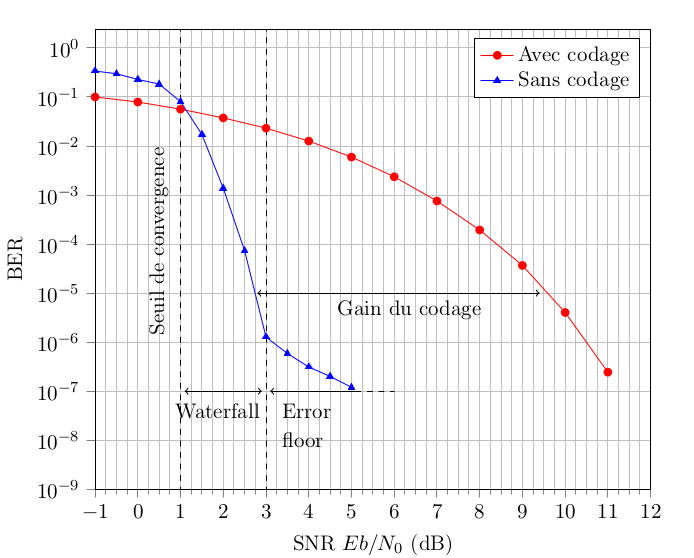
\includegraphics[scale=0.5]{chapter2/figs/comp_courbes_text.png}
    \caption{Évaluation des performances d'un CCE}
    \label{comp_codes}
\end{figure}

Dans la section suivante, nous présenterons de manière concise les principales familles de CCE actuellement utilisées dans les standards de communications numériques ainsi que les propriétés des algorithmes de décodage qui leur sont associées.
%
%
%
%
\section{Les différentes familles de CCE}
%
%
%
%
L’intégration des CCE dans les systèmes numériques a débuté dans les années 1950 par l’intégration des codes de Hamming \cite{Ham50}, qui ont été les premiers CCE proposés dans la littérature. Ces derniers sont des codes correcteurs linéaires qui utilisent quelques bits de redondance pour protéger l’information binaire, permettant ainsi de détecter et de corriger une fraction d'erreurs. Les recherches dans ce domaine se sont poursuivies et ont permis l'émergence des codes de Reed-Solomon dans les années 1960, ainsi que celle des codes convolutifs dans les années 1970. Ces deux familles améliorent fortement le pouvoir de correction des codes de Hamming au prix d’une augmentation notoire de la complexité calculatoire des algorithmes mis en œuvre pour leur décodage. Ces derniers ont été mis en application dans les premières générations de systèmes de communications numériques sans fils terrestres, mais aussi dans le domaine spatial. Toutefois, ils ont été remplacés dans les années 1990-2000 par de nouvelles familles de codes plus performantes telles que, par exemple, les turbo codes et les codes LDPC. Ces familles de codes, associées aux codes polaires et les codes LDPC non binaires, sont d'usage aujourd'hui dans des standards usuels tels que la 4G \cite{4G}, et la 5G \cite{5g}, ainsi que dans les standards de communications numériques par satellites \cite{DVB:RCS,CCSDS:NB,CCSDS,DVB:S2x}. Cet engouement autour de ces quatre familles est dû aux compromis intéressants qu’elles offrent en termes de pouvoir de correction et de complexité calculatoire.
%
%
%
%
\subsection{Les turbo codes}
%
%
%
%
Les turbo codes sont une classe de CCE découverte au début des années 1990  \cite{NearShanon, BookCodes}. Le développement de ces codes est fondé sur l'utilisation de deux codes convolutifs parallèles appelés codes composants, combinés par un processus d'encodage itératif. Ces derniers fonctionnent de manière complémentaire et exploitent l'interférence mutuelle pour améliorer les performances de correction d'erreurs. 
Les turbo codes ont permis d’obtenir des performances de décodage proches de la limite théorique de Shannon. 
En plus de leurs excellentes performances de décodage, la complexité calculatoire modérée de ces algorithmes et donc de leurs réalisations matérielles \cite{TURBO:TEN}, a accéléré leur inclusion dans de nombreux standards au début des années 2000 tels que les standards 3G \cite{3G}, 4G \cite{4G}, et 4G LTE \cite{Ref_4G}. Ils ont aussi été utilisés dans le domaine des communications satellitaires  \cite{CCSDS:TURBO,DVB:RCS}.
Depuis leur découverte, ces codes ont été étudiés avec attention  \cite{TURBO:SURVEY} afin d’améliorer leurs niveaux de performances: 
\begin{itemize}
    \item[(a)] en réduisant l’apparition des planchers d’erreurs  \cite{TURBO:NEW:INTERL} ;
    \item[(b)] en proposant des stratégies de parallélisation des algorithmes de décodage pour monter en débit  \cite{TURBO:ALGO1,TURBO:PIPE} ;
    \item[(c)] en concevant des architectures efficaces matériellement et énergétiquement pour faciliter leur intégration dans des systèmes embarqués contraints \cite{TURBO:HARD1,TURBO:HARD2,TURBO:HARD3}.
\end{itemize} 

\begin{figure}[b]
    \centering
    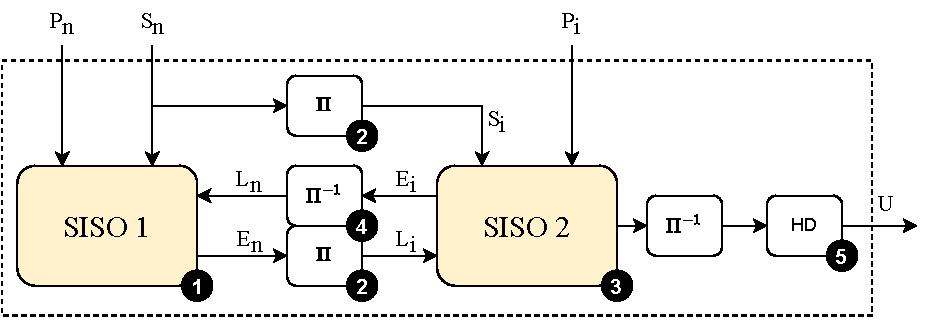
\includegraphics[scale=1]{chapter2/figs/siso_turbo.pdf}
    \caption{Structure d’un décodeur de turbo code }
    \label{TURBO1}
\end{figure}

Le processus de décodage associé aux turbo codes est schématisé dans la figure \ref{TURBO1}. De manière concise, les informations provenant du canal de communication notées ($\bm{S_n, P_n, P_i}$) sont traitées de manière itérative dans le récepteur. Dans un premier temps, les vecteurs d’information $\bm{S_n}$ et les données redondantes $\bm{P_n}$ sont traitées par le premier \acrshort{siso} (\ding{182} figure \ref{TURBO1}). Cette étape produit un vecteur de données extrinsèques $\bm{E_n}$, informations qui sont ensuite entrelacées par $\bm{\Pi}$ afin de produire le vecteur $\bm{L_i}$ (\ding{183} figure \ref{TURBO1}). Dans un second temps, les données $\bm{S_i, P_i, L_i}$ sont traitées de manière similaire par le second SISO (\ding{184} figure \ref{TURBO1}). Ce traitement produit les extrinsèques $\bm{E_i}$ qui post-entrelacement deviennent $\bm{L_n}$. L’exécution séquentielle des SISO \ding{182} et \ding{184} est réalisée $\bm{i}$ fois au maximum, ou jusqu’à obtention d’un mot de code valide en sortie du décodeur $\bm{U}$. Une formulation algorithmique du processus de turbo décodage est proposée dans l’Algorithme \ref{algo:turbo} avec $\bm{\Pi}$ et $\bm{\Pi^{-1}}$ les opérations d’entrelacement et de désentrelacement \cite{TURBO:NEW:INTERL}.

\begin{algorithm}[tb]
    \small
    \begin{algorithmic}[1]
        \State {\textbf{Step 1}: Chargement des données}
        \State $S_i$ = $\Pi$( $S_n$ )
        \State $E_i$ = zeros( $E_i$ )
        \item[]
        \State {\textbf{Step 2}: Décodage itératif}
        \ForAll{$t = 0 \to (iter\_max-1)$}
        \State $E_n$ = SISO( $P_n$, $S_n$, $E_i$ )
        \State $E_n$ = $\Pi$ ( $E_n$ )
        \State $E_i$ = SISO( $P_i$, $S_i$, $E_i$ )
        \State $E_i$ = $\Pi^{-1}$( $E_i$ )
        \EndFor
        \item[]
        \State {\textbf{Step 3}: Décision dure}
        \State $u_n$ = Décision dure( $P_n$, $S_n$, $E_i$ )
        \end{algorithmic}
    \caption{Formulation conventionnelle de l'algorithme de décodage turbo}
    \label{algo:turbo}
\end{algorithm}


Les traitements nommés SISO (Soft-Input, Soft-Output), utilisés dans la figure \ref{TURBO1}, sont des traitements œuvrant sur un treillis construit à partir des spécifications du turbo code \cite{BookCodes}. Pour identifier la séquence la plus probable dans le treillis constitué de $\bm S$ états figure \ref{TURBO2}, des algorithmes de type BCJR \cite{BCJR} sont utilisés. L'algorithme BCJR parcourt le treillis dans les deux sens afin d’estimer le chemin le plus probable à partir de cette estimation et de calculer les $\bm K$ valeurs extrinsèques.

\begin{figure}
    \centering
    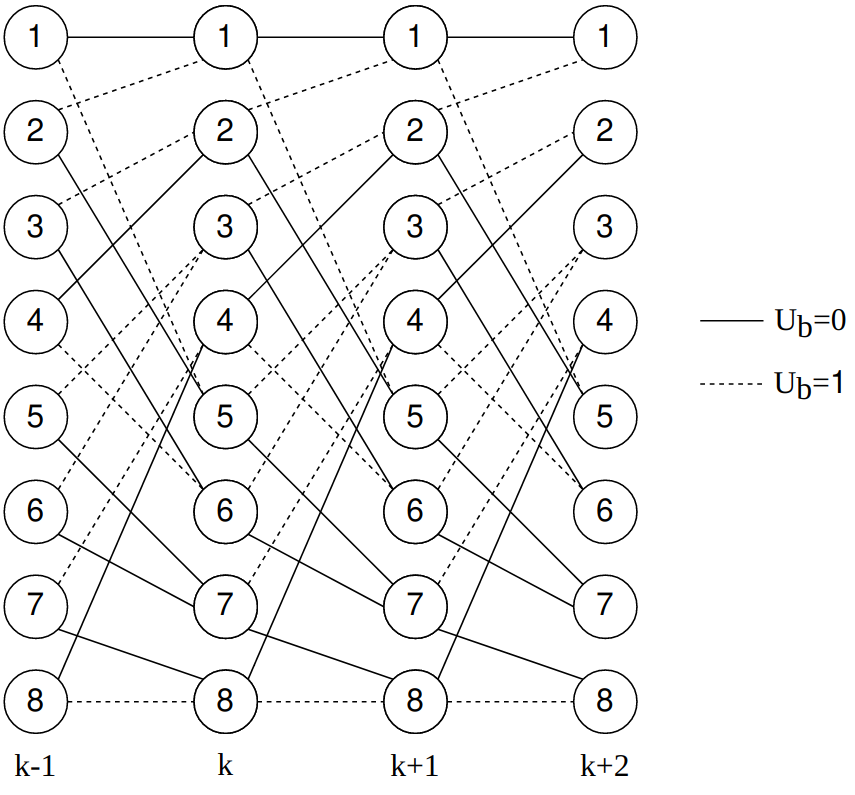
\includegraphics[scale=0.3]{chapter2/figs/turbo_treillis.png}
    \caption{Exemple de treillis à 8 états pour turbo code}
    \label{TURBO2}
\end{figure}


L’algorithme privilégié pour réaliser ce calcul au niveau du treillis lors de l’implantation temps réel de turbo décodeurs est l’algorithme BCJR Max-Log-MAP \cite{BCJR2}, car les opérations arithmétiques mises en œuvre sont peu complexes. Toutefois, il est à noter que ce dernier réduit légèrement les performances de décodage.
Ce traitement, dont la complexité calculatoire domine dans le décodeur, est composé de boucles itératives calculant séquentiellement les métriques internes au processus ($ \bm{\alpha}, \bm{\beta}, \bm{\gamma}$) afin de produire $\bm{K}$ informations extrinsèques. Ces calculs impliquent des accès irréguliers en mémoire liés à la structure du treillis.

\begin{algorithm}[tb]
\small
    \begin{algorithmic}[1]
        \For {Toutes les frames}
            \For {$k=0; k < K ; k=k+1$}
            \State $\gamma^k$ \leftarrow \textit{calculGamma} $(l^k_{sys},l^k_p,l^k_e)$ 
            \EndFor
            \State $\alpha^0$ \leftarrow \textit{initAlpha()}
            \For {$k=0; k < K ; k=k+1$}
            \State $\alpha^k$ \leftarrow \textit{calculAlpha} $(\alpha^{k-1},\gamma^{k-1})$ 
            \EndFor
            \State $\beta^{K-1}$ \leftarrow \textit{initBeta()}
            \For {$k=K-2; k \geq 0; k = k-1$}
            \State $\beta^k$ \leftarrow \textit{calculBeta} $(\beta^{k+1},\gamma^{k})$ 
            \EndFor
            \For {$k=0; k < K, k = k+1$}
            \State $L^k_e$ \leftarrow \textit{calculExtrinsèque}$(\alpha^k,\beta^k,\gamma^k)$ 
            \EndFor
        \EndFor
        \end{algorithmic}
    \caption{Implémentation standard du BCJR}
    \label{algo:ref}
\end{algorithm}

Afin de rendre le processus de décodage des turbo codes compatible avec les contraintes temps réel, différents verrous ont dû être levés  \cite{TURBO:TEN,TURBO:SURVEY}. Tout d’abord, dans le but d'atteindre des débits compatibles avec les besoins applicatifs, différentes stratégies de parallélisation du parcours du treillis ont été proposées tout comme l’exécution parallèle des SISO \cite{TURBO:HARD3}.

Toutefois, de manière à permettre l’implantation temps réel de turbo décodeurs dans des contextes contraints en termes d’énergie et de débit \cite{TURBO:HARD2}, de nombreuses solutions ont été proposées pour simplifier les algorithmes de décodage \cite{TURBO:SURVEY} mis en œuvre et augmenter la parallélisation des calculs \cite{TURBO:ALGO1}. Ces avancées ont permis l’intégration des turbo codes dans la 3G \cite{3G}, la 4G LTE \cite{Ref_4G} et potentiellement leur usage dans la 5G/6G \cite{5g,Ref_6G} ou les standards associés à l’IoT \cite{ref_trubo_6g}.
En parallèle des travaux menés autour des turbo codes, d’autres familles de codes correcteurs, tels que les codes LDPC, ont aussi émergé grâce à leur excellent pouvoir de correction. 

% 
% 
% 
\subsection{La famille des codes LDPC binaires}
% 
% 
% 
Les codes LPDC (Low Density Parity Check) sont proposés pour la première fois par Robert G. Gallager au début des années 1960 \cite{LDPC1}. À l’origine, malgré l’intérêt de la communauté pour ses travaux, la complexité calculatoire induite par le processus de décodage était trop importante vis-à-vis des capacités d’intégration. Il fallut attendre la fin des années 1990, et les progrès technologiques réalisés dans le domaine de l’intégration des circuits numériques pour que ces travaux soient exhumés par MacKay \cite{LDPC2}. Comme les turbo codes, les codes LDPC possèdent un pouvoir de correction proche de la limite de Shannon \cite{LDPC2}. Les algorithmes de décodage mis en œuvre sont aussi itératifs et possèdent des complexités calculatoires modérées \cite{LDPC3,LDPC4}. Toutefois, contrairement aux turbo codes cette famille de CCE qui n’était pas protégée par des brevets, a généré un engouement dans la communauté scientifique, tant sur les aspects théoriques liés à la construction des codes et leur décodage, que sur la conception de circuits numériques efficaces en termes de débit, d'énergie et de latence.
Ainsi, un nombre important de travaux de recherche se sont focalisés sur la conception de codes LDPC, que l’on nomme parfois matrices de parité, efficaces \cite{LDPC5, LDPC6} pour la simplification des algorithmes de décodage \cite{LDPC:MS} et la conception d’architectures matérielles dédiées \cite{Hailes2016}. Les avancées significatives dans ces domaines, associées aux besoins de montée en débit des systèmes de communications numériques, ont abouti à l’inclusion en 2005 des codes LDPC dans les standards WiMAX \cite{Ref_Wimax} et DVB-S2 \cite{DVB:S2}. Ces standardisations ont amplifié l’intérêt des communautés universitaires et industrielles pour cette famille de CCE, engendrant ensuite son adoption dans les standards DVB-S2X \cite{DVB:S2x} et CCSDS \cite{CCSDS}. Plus récemment, les codes LDPC ont aussi été adoptés dans le standard 5G \cite{5g} pour assurer la protection des paquets de données. 
Les codes LDPC, sont des codes linéaires en blocs définis à l’aide de matrices de parité de faible densité nommées \textbf{H}. Ces matrices, dont un exemple est présenté dans l’équation \ref{Eq21}, sont composées de \textbf{N} colonnes et de $\bm{M=N-K}$ lignes. À l’émission, un vecteur \textbf{x} de \textbf{N} bits est généré pour transmettre \textbf{K} bits d’information à l’aide d’une matrice génératrice nommée $\bm{G=H^{-1}}$. Si l'on considère qu'un vecteur $\bm{\lambda}$ composé de \textbf{N} informations bruitées est reçu après le passage des données par le canal de transmission, les \textbf{M} équations de parité issues de \textbf{H} sont utilisées à la réception pour détecter et corriger les erreurs présentes dans $\bm{\lambda}$. Les \textbf{N} colonnes et les \textbf{M} lignes de \textbf{H} représentent respectivement les nœuds variables ($\bm{V_n}$) et les nœuds de vérification de parité ($\bm{C_n}$). Pour chaque élément non nul de \textbf{H}, il existe une dépendance entre les éléments $\bm{V_n}$ et $\bm{C_n}$. Le nombre d’éléments de la ligne $J$ et de la colonne $I$ de \textbf{H} sont respectivement les degrés de $\bm{C_n}$ et $\bm{V_n}$, notés $\bm{D_c}(j)$ et $\bm{D_v}(i)$ pour un code LDPC($\bm{D_c}$, $\bm{D_v}$).

\begin{equation}
\mathbf{H}=
\begin{blockarray}{ccccccccc}
     & \bm{V_0} & \bm{V_1} & \bm{V_2} & \bm{V_3} & \bm{V_4} & \bm{V_5} & \bm{V_6} & \bm{V_7} \\
    \begin{block}{c(cccccccc)}
      \bm{C_0} & 1  & 1  & 1  & 1  & 0  & 0  & 0  & 0 \\
      \bm{C_1} & 0  & 0  & 0  & 1  & 1  & 1  & 0  & 0 \\
      \bm{C_2} & 0  & 1  & 0  & 0  & 1  & 0  & 1  & 1 \\
      \bm{C_3} & 1  & 0  & 0  & 1  & 0  & 0  & 1  & 0 \\
      \bm{C_4} & 1  & 0  & 1  & 1  & 0  & 0  & 1  & 0 \\
    \end{block}
    \end{blockarray}
\label{Eq21}
\end{equation}

Les matrices \textbf{H} peuvent être représentées de manière visuelle à l’aide de graphes bipartites nommés graphes de Tanner \cite{Tanner}. Par exemple, le graphe de Tanner représenté en figure \ref{Tanner} est équivalent au code LDPC (8,5) décrit dans l’équation \ref{Eq21}.

\begin{figure}
    \centering
    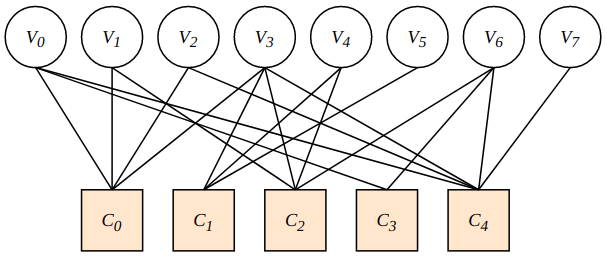
\includegraphics[scale=0.5]{chapter2/figs/tanner.png}
    \caption{Représentation d’un code LDPC sous forme d’un graphe de Tanner}
    \label{Tanner}
\end{figure}

Dans leur forme générale  \cite{Gallager62,LDPC2}, les matrices \textbf{H} sont irrégulières et non-structurées. Cependant, la conception de décodeurs efficaces pour un code LDPC non-structuré est admise par tous comme étant une tâche ardue \cite{NISC:BLG}. Ainsi, pour faciliter la conception de décodeurs LDPC temps réel, qu’ils soient matériels ou logiciels, les codes LDPC Quasi Cycliques (QC-LDPC) ont été adoptés dans la majorité des standards \cite{wifi, wimax, wlan, verizon}, y compris pour le standard 5G 3GPP  \cite{5g}. Cette sous-famille des codes LDPC, permet de garantir un niveau de parallélisme constant durant le processus de décodage ainsi que l’absence de conflits d’accès à la mémoire. Pour procurer ces caractéristiques, les codes LDPC-QC \cite{QC:LDPC} de taille $\bm{N \times M}$ sont structurés à partir de sous matrices de taille $\bm{Z \times Z}$.


Pour décoder les codes LDPC, les algorithmes de type passage de messages (MP, message passing) sont habituellement utilisés. L’algorithme de référence en termes de pouvoir de correction est l’algorithme somme-produit (SPA) détaillé dans \cite{LDPC:SPA}. Le principe général de décodage est le suivant : à partir des valeurs des informations en provenance du canal ($\bm{V_n}$), des messages $\bm{V_n}$  \rightarrow $\bm{C_n}$ sont calculés, puis transmis aux nœuds de parité ($\bm{C_n}$). Ces nœuds de parité, en fonction de leur validation ou non, retournent des messages ($\bm{C_n}$ \rightarrow $\bm{V_n}$) vers les nœuds $\bm{V_n}$ afin de confirmer ou d’infirmer les données reçues. Le processus de décodage est itératif, il s’arrête lorsque tous les nœuds $\bm{C_n}$ sont validés, ou bien lorsqu’un nombre maximal d’itérations a été réalisé.

La nature des opérations réalisées dans l’algorithme SPA original \cite{LDPC:SPA} ainsi que l’ordonnancement des calculs n’étaient pas adaptés à l’implémentation de décodeurs temps réel. Des simplifications algorithmiques permettant l’abandon des fonctions transcendantales et le passage en virgule fixe du processus de décodage ont été proposés dans \cite{LDPC:APPROX:1,LDPC:APPROX:2,LDPC:APPROX:3,LDPC:APPROX:4,LDPC:ARCH2}. Ces variantes algorithmiques regroupées sous la dénomination générique d’algorithmes \textit{Min-Sum} ont ensuite bénéficié d’une modification de l’ordonnancement des calculs lors du processus de décodage, passant d’une approche par vagues en deux phases (TPMP – two phase message passing) à une approche par couches horizontales (HL – horizontal layered schedule) \cite{LDPC:HL}. Cette modification de l’ordonnancement des calculs permet de réduire d’environ $\mathit{2/5}$ la complexité mémoire et de diviser, approximativement, par deux le nombre d’itérations de décodage à iso-performances. Ces caractéristiques avantageuses ont entrainé une utilisation de la stratégie HL dans les décodeurs LDPC récents, qu’ils soient matériels \cite{LDPC:APPROX:3,LDPC:APPROX:4,LDPC:ARCH1,LDPC:ARCH2} ou logiciels \cite{LDPC:SOFT1,LDPC:SOFT2,LDPC:SOFT3,LDPC:SOFT4}.
\begin{algorithm}
{
	\small
	\begin{algorithmic}[1]
		\Statex {\textbf{Kernel 1}: Initialisation}
		\State Charge la trame dans la mémoire dédiée au VN
		\ForAll{$m \in \Psi, n \in \Phi(m)$}[\textit{$\Psi$ est l'ensemble des CNs}] %\COMMENT{$\Psi$ est l'ensemble des CNs}
		\State Initialisation de la mémoire message : $\mathcal{L}^{(0)}_{mn}=0$
		\EndFor
		\State {\textbf{Kernel 2}: Traitement des \textit{Imax} itérations de décodage}
		\ForAll{$i = 1 \to (Imax)$}
		\ForAll{$m \in \Psi$}[\textit{Pour tout CN}] %\COMMENT{Pour tout CN }
			
		\State {\textbf{Kernel 3.1}: Calcul des messages entrants $\mathcal{L}_{nm}$ }
		\ForAll{$n \in \Phi(m)$}[\textit{VNs contribuant à CN}] %\COMMENT{VNs contribuant à CN}
		\State $ \mathcal{L}^i_{nm} = \textit{VN}_n - \mathcal{L}^{(i-1)}_{mn} $
		\EndFor

		\State {\textbf{Kernel 3.2}: Génération des messages sortants $\mathcal{L}_{mn}$ }
		\ForAll{$n \in \Phi(m)$}
		\State $sign(\mathcal{L}^i_{mn}) = \left[ \displaystyle\prod_{n'\in \Phi(m)/n} sign(\mathcal{L}^{(i-1)}_{n'm}) \right]$
		\State $|\mathcal{L}^i_{mn}| = \left[ \displaystyle\min_{n'\in \Phi(m)/n} |\mathcal{L}^{(i-1)}_{n'm}| \right]$
		\EndFor
			
		\State {\textbf{Kernel 3.3}: Mise à jour des VNs}
		\ForAll{$n \in \Phi(m)$}
		\State $ \textit{VN}_n = \mathcal{L}^{(i)}_{nm} + \mathcal{L}^{(i)}_{mn} $
		\EndFor
			
		\EndFor
		\EndFor
			
		\State {\textbf{Kernel 4}: Décision dure sur chaque LLR de la trame}
		\ForAll{$n \in trame$}
		\State $ c_n = \begin{cases}
                   0,& \text{if } \textit{VN}_n \leq 0\\
                   1,& \text{if } \textit{VN}_n > 0
               \end{cases} $
       \EndFor            
	\end{algorithmic}
	}
	\caption{\small Algorithme Min-Sum basé sur un ordonnancement par couches horizontales}
	\label{ldpc_minsum}
\end{algorithm}

L’Algorithme \ref{ldpc_minsum} présente la formulation d’un algorithme de décodage LDPC dans lequel l’approximation \textit{Min-Sum} est couplée avec un ordonnancement par couche horizontale $\bm{C_n}$ \cite{LDPC:HL}. Cette formalisation de l’algorithme de décodage met en évidence la structuration du processus de décodage en nids de boucles sur 3 niveaux. Différentes stratégies de parallélisation ont été proposées et mises en œuvre pour accélérer l’implantation du processus de décodage:
\begin{itemize}
    \item les kernels internes (3.1, 3.2, 3.3) qui ont des nombres d'itérations variables en fonction du degré des nœuds $\bm{C_n}$ peuvent être déroulées ou partiellement déroulées pour certains codes.
    \item le kernel (3) peut être déroulé partiellement d’un facteur \textbf{Z} dans le cas de codes LDPC QC. Un déroulage partiel plus important est difficile à obtenir à cause des dépendances de données liées à la structure de la matrice \textbf{H}.
    \item Le kernel (2) doit quant à lui itérer séquentiellement $\mathit{i}$ fois à cause des dépendances de données entre les itérations. 
\end{itemize}

L'exploitation de ces différents niveaux de parallélismes associés à des contraintes applicatives spécifiques, a permis la conception d’architectures numériques variées permettant d’atteindre des débits de plusieurs Gbps sur technologies \acrshort{fpga} \cite{PIGNOLY:MS,BOUTILLON}, mais aussi d’atteindre des débits similaires sur des architectures programmables \cite{LDPC:SOFT4,FAIR:LDPC}. \\
L’ensemble de ces solutions ont permis d'obtenir des compromis \textit{débit vs flexibilité}, permettant l’émergence et l’usage à grande échelle des plateformes SdR \cite{SDR, SURVEY:SDR} et des systèmes de type Cloud-RAN \cite{CLOUD:RAN2,CLOUD:RAN3} plébiscités par exemple pour le déploiement de la 5G \cite{CLOUD:RAN1}. 

En supplément des travaux relatifs à la construction des codes LDPC et de l’amélioration des caractéristiques des décodeurs matériels et logiciels, d’autres initiatives se sont focalisées sur l’extension de cette famille aux corps de Galois non binaires ($\mathbb{GF}( \bm{q} )$ avec $\bm{q}\ge2$).

% OK
% 
% 
% 
% 
\subsection{La famille des codes LDPC non binaires (LDPC-NB)}
% 
% 
% 
% 
Les codes LDPC binaires offrent des performances de décodage proches de la limite de Shannon lorsque la taille des trames est suffisamment grande (\textbf{N} > 1000). Cependant, dans de nombreux domaines applicatifs, cette condition n’est pas remplie, car les systèmes échangent peu d’informations et nécessitent des latences faibles, impliquant de fait l’usage de trames courtes. \\
Pour améliorer les performances de décodage dans ces conditions, une extension des codes LDPC binaires au corps de Galois avec ($\mathbb{GF}(\bm{q})$ avec $\bm{q} \ge 2$ a été proposée dans \cite{NBLDPC:1,NBLDPC:2}. L’utilisation de corps de Galois non binaires permet d’augmenter la diversité et de lutter contre les cycles courts dans les codes. 

L’utilisation de corps de Galois avec $\bm{q} \in{\{16, 64, 256\}}$ permet d’améliorer le pouvoir de correction de 1,0 dB à 1,3 dB face à des codes LDPC binaires de tailles équivalentes, comme cela est démontré dans \cite{CCSDS:NB,NBLDPC:3}. Toutefois, l’amélioration notable des performances de décodage est obtenue au prix d’une augmentation polynomiale de la complexité calculatoire \cite{NBLDPC:1}. \\
Par conséquent, un nombre important de travaux tels que \cite{survey:NB} se sont concentrés sur cette nouvelle famille de codes. Un code NB-LDPC \textbf{(N, K)} est un code en bloc linéaire défini par une matrice de parité de taille \textbf{M×N} appelée \textbf{H}, dont les éléments non-nuls appartiennent à ($\mathbb{GF}(\bm{q})$ comme cela est présenté dans l’équation \ref{YYW} ci-dessous pour $\bm{q}$ = 128.



\begin{equation}
\mathbf{H}=
\begin{blockarray}{ccccccccc}
     & \bm{V_0} & \bm{V_1}  & \bm{V_2}    & \bm{V_3}    & \bm{V_4}    & \bm{V_5} & \bm{V_6} & \bm{V_7} \\
\begin{block}{c(cccccccc)}
  \bm{C_0} & \alpha_{00}    & \alpha_{10} & \alpha_{20}  & 0          &        0  & 0  & 0  & 0 \\
  \bm{C_1} & 0              & 0           & 0           & \alpha_{31} & \alpha_{41}  & \alpha_{51}  & 0  & 0 \\
  \bm{C_2} & \alpha_{02}    & 0           & 0           & \alpha_{32} & 0         & 0  & \alpha_{62}  & 0 \\
  \bm{C_3} & 0              & \alpha_{13} & 0           &  0          & \alpha_{43}        & 0  & 0  & \alpha_ {73} \\
\end{block}
\end{blockarray}
\label{YYW}
\end{equation}

Contrairement aux codes LDPC binaires, les éléments $\bm{V_N}$ et $\bm{C_N}$ sont des symboles composés de $\bm{log_2(q)}$ bits. La modélisation sous la forme de graphe de Tanner de ces matrices met en évidence les opérations de multiplication et de division des messages $\bm{V_N}$ \rightarrow $\bm{C_N}$ et $\bm{C_N}$ \rightarrow $\bm{V_N}$ dans ($\mathbb{GF}$) lors de l’échange des messages, comme représenté dans la figure \ref{YYZ}.

\begin{figure}
    \centering
    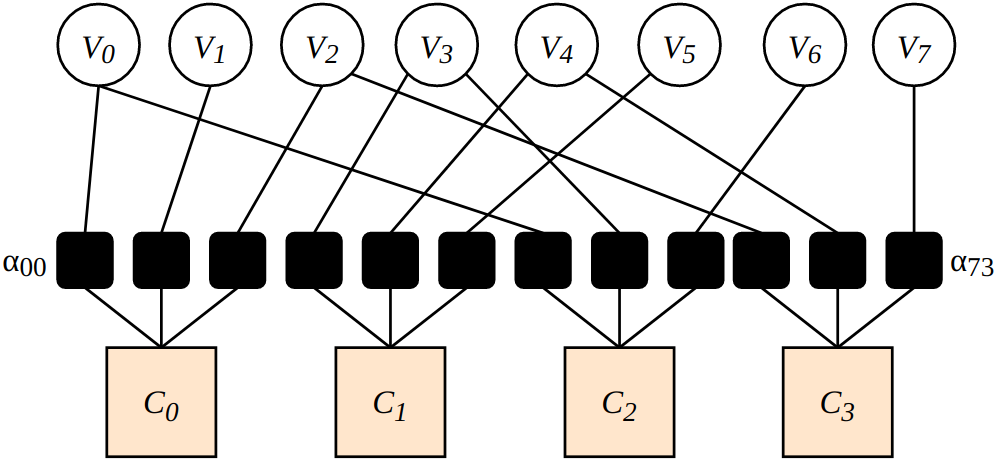
\includegraphics[scale=0.3]{chapter2/figs/yyz.png}
    \caption{Graphe de Tanner correspondant à la matrice LDPC-NB décrite dans l’équation \ref{YYW}.}
    \label{YYZ}
\end{figure}

Le décodage des codes NB-LDPC s’effectue grâce à l’utilisation d'algorithmes de passage de messages équivalents à ceux employés pour le décodage des codes LDPC binaires. Toutefois, les algorithmes employés sont plus complexes, principalement à cause de la nature des données échangées. En effet, les valeurs internes des nœuds $\bm{V_N}$ et $\bm{C_N}$ ne sont plus des données scalaires, mais des vecteurs composés de \textbf{q} valeurs de LLR. Il en va de même pour les messages échangés entre les différents nœuds. Les meilleures performances de correction sont obtenues en exécutant l'algorithme \textit{Sum-Product} (SPA) \cite{NB:SPA} ou sa reformulation FFT-SPA \cite{NB:SPA} qui réduit fortement la complexité calculatoire du processus de décodage à iso-performance.


% i : Vn 
% j : Cn 

% M i to j => messages Vn vers Cn 
% Pi(x) => LLRs du canal 
% psi : ensemble de J liées à i 

\begin{algorithm}[t]   
{
        \small
        \begin{algorithmic}[1]
            \Statex \textbf{Étape 1:} Initialisation
            \State $p_i(x)=p(v_i=x|y{-i})$
            \State $m^0_{ji}(x)=1$
            \Statex \space \triangleright \space Effectue le processus avec \textit{iter\_max} itérations 
            \ForAll{$t=1\rightarrow (iter\_max)$}
                \Statex \textbf{Étape 2:} Pour chaque $C_n$ du code LDPC-NB
                \ForAll{$j \in C$}
                    \State \space \triangleright \space Calcul les messages entrants $m_{ij}$
                    \ForAll{ $i \in \Psi (j)$ }
                        %\State $m^t_{ij} = \left(\displaystyle\sum_{x\in\mathbb{GF}} m^{t-1}_{ji}(x) \right)  \times \left(\frac{p_i(x)}{m^{t-1}_{ji}(x)}\right) $
                        
                        \State $m^t_{ij} = p_i(x) - m^{t-1}_{ji}(x) $
                        \State $m^t_{ij} = m^{t}_{ij} - min(m^t_{ij}) $ // <- min des GF 
                        \State $M^t_{ij} = \Theta_{\alpha_{ij}}(m^t_{ij})$
                        %\State $\tilde{M}^t_{ij} = FFT(M^t_{ij})$
                    \EndFor
                    \State \space \triangleright \space Noeuds parité, recherche du minimum dans le domaine $\mathbb{GF}$
                    \ForAll{$i \in \Psi(j)$} 
                        %\State $\tilde{M}^t_{ji} = \displaystyle\prod_{i'\in\Psi(j)/i} \tilde{M}^t_{i'j}$
                        \State $\tilde{M}^t_{ji} = min \displaystyle\sum_{i'\in\Psi(j)/i} \tilde{M}^t_{i'j}$
                    \EndFor
                    \State \space \triangleright \space Calcul des messages $m_{ij}$ sortants
                    \ForAll{$i \in \Psi(j)$} 
                        %\State ${M}^t_{ji} = FFT^{-1}(\tilde{M}^t_{ji})$
                        \State $m^t_{ji} = \Theta_{\alpha_{ij}}^{-1} (M^t_{ji})$
                    %\EndFor
                    %\State \space \triangleright \space Mise à jour des symboles
                    %\ForAll{$i \in \Psi(j)$}
                        %\State $p_i(x) = p_i(x) \times \left(\frac{m^t_{ji}(x)} {m^{t-1}_{ji}(x)}\right) $
                        \State $ p_i(x) = p_i(x)+ m^t_{ji} $
                    \EndFor
                \EndFor
            \EndFor
            \Statex \textbf{Étape 3:} Décision dure des symboles
            \ForAll{$i \in V$}
                \State $\hat{v}_i = arg \space max \space (p_i(x))$
            \EndFor
        \end{algorithmic}
    }
    \caption{\small Algorithme horizontal TPMP Min-Sum}
    \label{algo:ldpcnb_fftspa}
\end{algorithm}


L'algorithme \ref{algo:ldpcnb_fftspa} présente une formalisation de l'algorithme de décodage \textit{Min-Sum} basée sur un ordonnancement horizontal des calculs de parité \cite{NB:FFT:BLG}. Cet ordonnancement des calculs de parité permet d’obtenir une accélération de la convergence du processus de décodage et diminue la complexité mémoire.\\
L'algorithme \ref{algo:ldpcnb_fftspa} met en évidence une structure en nids de boucle, proche de celle présente dans les algorithmes des décodages des codes LDPC binaires (algorithme \ref{ldpc_minsum}). Toutefois, la complexité calculatoire et le parallélisme de calcul présents ici sont localisés au sein des kernels qui ne manipulent plus des données scalaires, mais des vecteurs de données dont la taille est proportionnelle à $2^{\mathbb{GF}}$. 
L'algorithme est inspiré des travaux détaillées dans \cite{NB:FFT:BLG,14,15,16}, proposant un algorithme FFT-SPA adapté à une exécution sur des cibles programmables multicœurs et many-cœurs.\\
Des variantes algorithmiques \cite{17,18,19} supportant le codage des données en virgule fixe sur un faible nombre de bits ont été élaborées à partir de l’algorithme de décodage SPA. Ces variantes nommées \textit{Min-Sum} (MS), \textit{Min-Max} (MM) et \textit{Extended Min-Sum} (EMS) ont permis par la suite le développement de décodeurs matériels dédiés \cite{22,21}, atteignant de hauts débits avec des complexités matérielles maîtrisées. Cependant, ces niveaux élevés de performance démontrés par ces architectures dédiées ont été obtenus au prix d’une réduction drastique de la flexibilité des décodeurs et nécessitent en amont de nombreuses étapes de simplification du décodeur vis-à-vis du code à traiter, étapes qui peuvent s’avérer chronophages \cite{phd_hassan}.

Les gains de codage fournis par cette famille de codes pour des courtes trames, combinés à leur capacité à s’associer avec des modulations d’ordre élevé ainsi que l’émergence de solutions d’implantations efficaces, ont motivé son introduction dans plusieurs standards spatiaux CCSDS \cite{CCSDS:NB}, BeiDou Navigation System \cite{BEIDOU} ainsi que son usage par exemple, dans le projet ANR QCSP \cite{phd_moniere,phd_kassem} pour le domaine des communications IoT.

%
% 
%
% 
% 
\subsection{La famille des codes polaires}
% 
%
%  
% 
Les codes polaires proposés en 2008 par Arikan \cite{Arikan08} sont des codes linéaires en blocs dont la taille des blocs $\bm{N}$ évolue en $2^{\bm{n}}$ avec $\bm{n}$ un nombre entier. Ces codes permettent d’atteindre théoriquement des performances proches de la capacité sur un canal gaussien lorsque $\bm{N}$ tend vers l’infini. 
Afin d’étudier leurs performances de décodage lorsque $\bm N < \infty$ et les comparer aux décodeurs développés pour les turbo codes et les codes LDPC, de nombreux travaux de recherche ont été menés durant la dernière décennie \cite{Golden,phd_seyyed}. 

L’algorithme de décodage initial nommé Successive Cancellation (SC) \cite{89,97} a mis en évidence la faible complexité calculatoire du processus de décodage. Cependant, l’écart de performance en termes de pouvoir de correction avec les autres familles de CCE a motivé la proposition d’algorithmes plus complexes tels que le Simplified-SC \cite{91, 92, 101}, le SC-List \cite{87, 122}, le SC-Stack \cite{SC:STACK}, le SC-Flip \cite{85, 86} et le SC-SCAN \cite{SC:SCAN}.

Ces derniers, au prix de complexités calculatoires plus importantes, permettent de compenser cette faiblesse et d'approcher et égaler les performances décodeurs LDPC et des turbo codes. En parallèle, différentes architectures de décodeurs décrites au niveau RTL ont été détaillées dans la littérature \cite{88, 89, 90, 91, 92, 93} afin de montrer la viabilité de ces algorithmes de décodage. Ces diverses avancées ont abouti leur inclusion en 2017 dans le standard 5G \cite{5g}, en remplacement des turbo codes, pour la protection des canaux de contrôle.


Le processus de codage côté émetteur consiste à multiplier la matrice de Kronecker \cite{Arikan08} par un vecteur $\bm{ \hat{u} }$ de \textbf{N} bits contenant \textbf{K} bits d’information et $\bm{M=N-K}$ bits gelés. Ces bits gelés dont les positions et les valeurs sont partagées par l’émetteur et le récepteur jouent le rôle de redondance. Le processus de décodage vise à faire successivement une estimation pour chaque valeur des bits $\bm{\hat{u}_i}$ sur la base des bits estimés précédemment $\bm{ \hat{u}_{ (0:i-1) }}$. Comme proposé dans \cite{Arikan_2009}, une représentation en \textit{Factor Graph} (FG) des codes polaires peut être utilisée pour représenter le calcul de $\bm{ \lambda_{0:i}}$. La figure \ref{XXPC} contient un exemple de \textit{factor graph} pour un code de largeur $\bm{N=8}$. Le décodeur estime successivement les bits $\bm{\hat{u}}$ à partir des données (LLR) provenant du canal et injectés à la droite du graphe.
%%%%%%%%%%%%%%%%%%%%%%%%%%%%%%
\begin{figure}
    \centering
    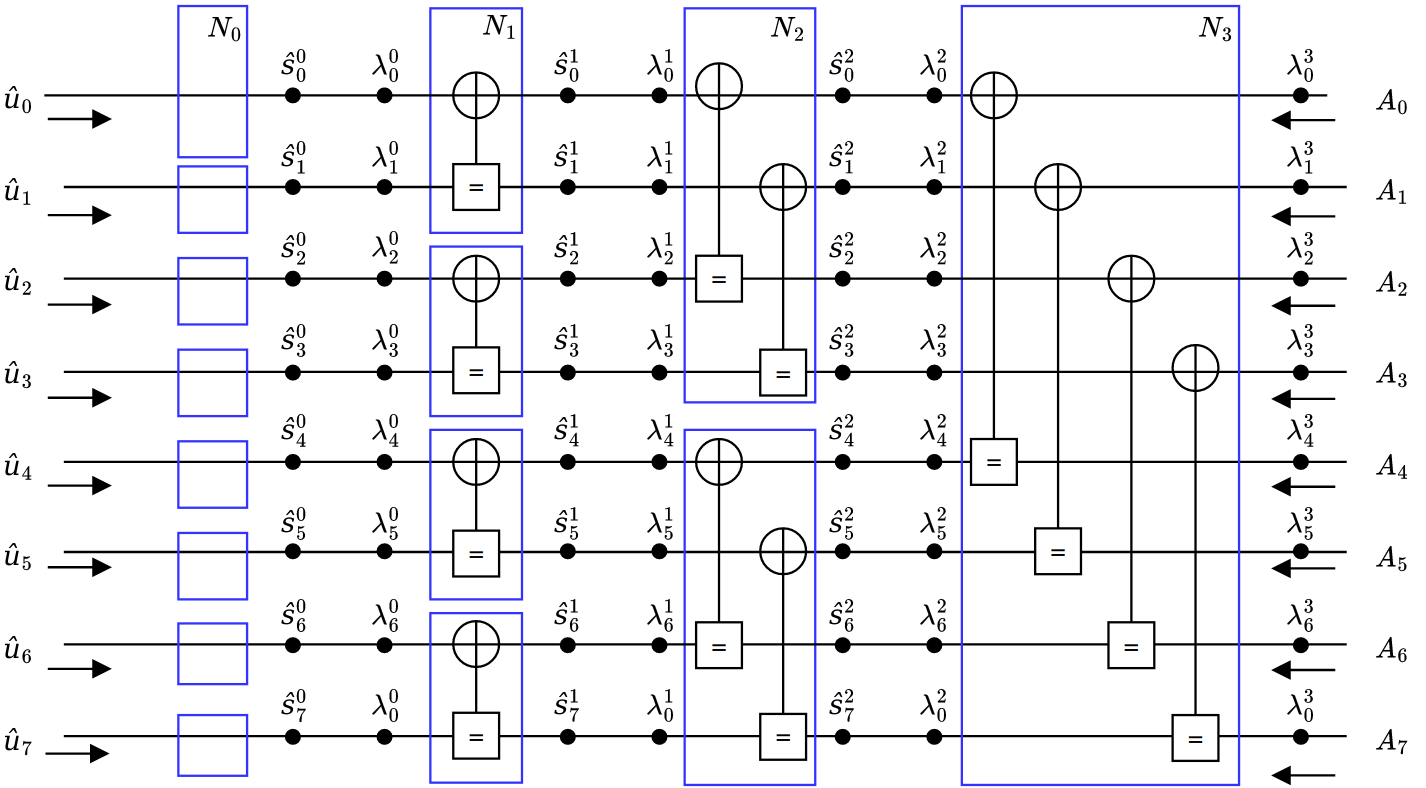
\includegraphics[scale=0.3]{chapter2/figs/XXPC.png}
    \caption{Représentation en factor graph du décodage SC d’un code polaire de taille N=8.}
    \label{XXPC}
\end{figure}
%%%%%%%%%%%%%%%%%%%%%%%%%%%%%%
La nature séquentielle de l’algorithme de décodage SC liée au calcul ordonné des sorties $\bm{\hat{u}}$ implique de fortes dépendances de données entre les nœuds. Cette caractéristique limite le parallélisme exploitable et génère un parallélisme de calcul, fluctuant en fonction des étapes, comme cela est mis en évidence par la taille des rectangles bleus dans la figure \ref{XXPC}. Afin de mieux mettre en évidence les dépendances de données ainsi que la variation du parallélisme de calcul, il est possible de modéliser le processus de décodage à l’aide d’un arbre binaire comme suggéré dans \cite{91}.
%%%%%%%%%%%%%%%%%%%%%%%%%%%%%%
\begin{figure}
    \centering
    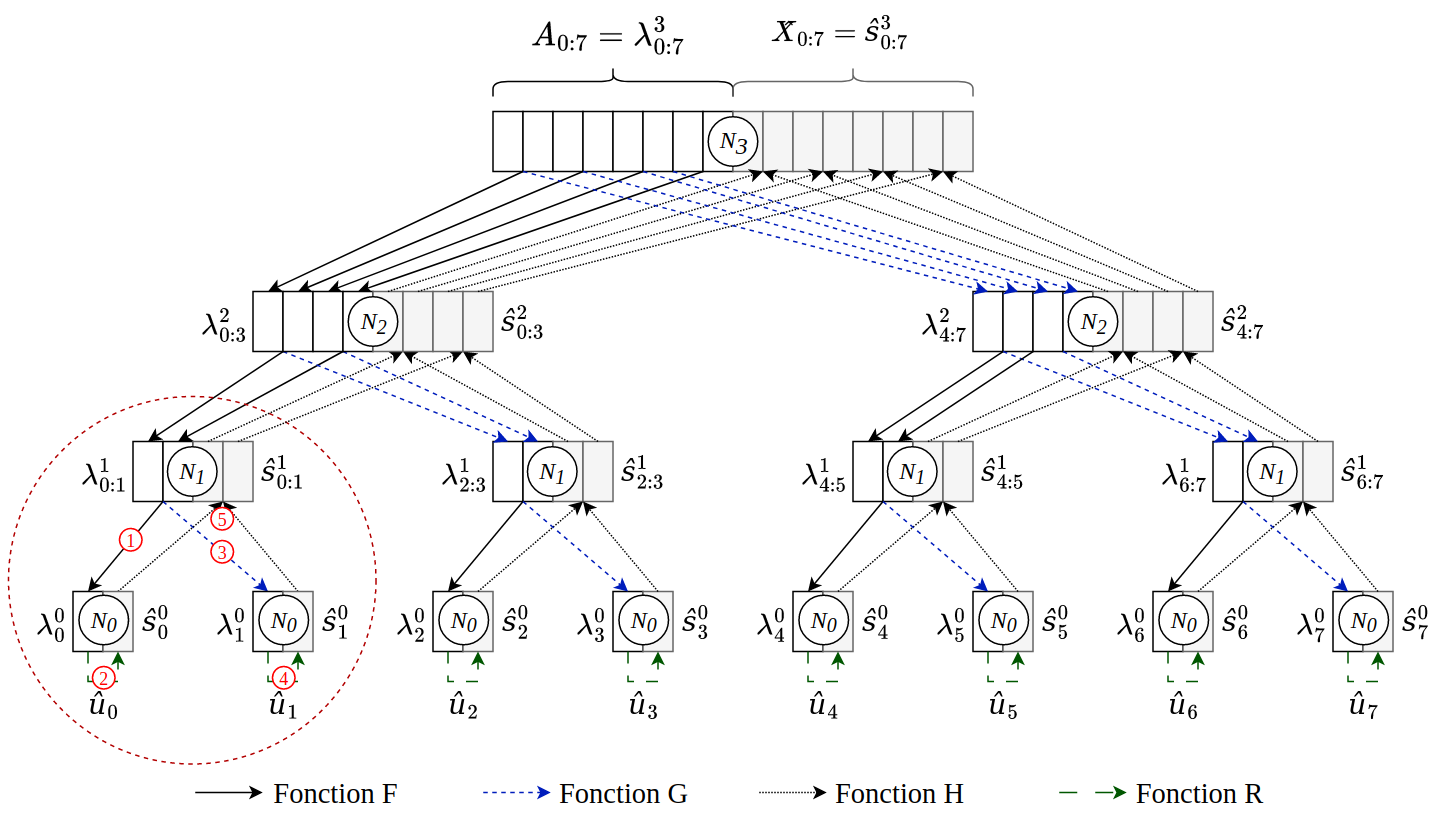
\includegraphics[scale=0.3]{chapter2/figs/ZZ.png}
    \caption{Représentation sous forme d’arbre du processus de décodage d’un \\décodeur polaire SC N=8}
    \label{ZZ}
\end{figure}
%%%%%%%%%%%%%%%%%%%%%%%%%%%%%%
Lors du décodage d’une trame composée \textbf{N} LLRs, l’arbre binaire représenté dans la figure \ref{ZZ} est parcouru de façon récursive depuis le nœud $\bm{(N_3)}$ de manière à produire l’ensemble des $\bm{N/2}$ sorties $\bm{\hat{u}_i}$. Le parcours de l’arbre binaire est opéré dans l’ordre suivant : du nœud racine vers le sous-nœud gauche puis vers le sous-nœud droit. Le nœud racine est situé au niveau $\bm{d = log(N)-1}$ et les nœuds feuilles sont les nœuds du niveau $\bm{d=0}$.
Le nœud racine $\bm{N_3}$ reçoit $\bm{N}$ valeurs de LLRs provenant du canal et échange successivement des données avec les sous-nœuds gauches et droits du niveau $\bm{N_2}$. Les nœuds feuilles $\bm{N_0}$ sont appelés par les nœuds $\bm{N_1}$ et ils génèrent l’estimation $\bm{\hat{u}_i}$. En supposant qu’un nœud non feuille/non racine $\bm{N_j}$ reçoit $\bm{\lambda_{a:a+J-1}}$, il exécute l’Algorithme itératif décrit dans l’Algorithme \ref{polar:algo}.
%%%%%%%%%%%%%%%%%%%%%%%%%%%%%%
\begin{algorithm}[tb]
    \begin{algorithmic}[1]
        \Statex \textbf{Nécessite:} $\lambda^j_{a:a+J-1}$ 
        \Statex \hspace{3mm} \textbf{Calcul $J/2$ fonctions $f$ concurrentes :}
        \State \hspace{3mm} $\lambda^{j-1}_i = f( \lambda^j_i; \lambda^j_{i+\frac{j}{2}}) , a \leq i \leq \frac{J}{2},$

        \Statex \hspace{3mm} \textbf{Appel récursif du noeud fils gauche $\mathcal{N}_{j-1}$}
        \State \hspace{3mm}  $\hat{s}^{j-1}_{a:a+\frac{J}{2}-1}=\mathcal{N}_j(\lambda^j_{a:a+J-1})$

        \Statex \hspace{3mm} \textbf{Calcul $J/2$ fonctions $g$ concurrentes :}
        \State \hspace{3mm} $\lambda^{j-1}_i = g( \lambda^j_{i-\frac{J}{2}} : \lambda^j_i:\hat{s}^{J-1}_{i-\frac{J}{2}}), a+\frac{j}{2}\leq i \leq J $

        \Statex \hspace{3mm} \textbf{Appel récursif du noeud fils droit $\mathcal{N}_{j-1}$}
        \State \hspace{3mm} $\hat{s}^{j-1}_{a+\frac{J}{2}:a+J-1} =\mathcal{N}_j(\lambda^{j-1}_{a+\frac{J}{2}:a+J-1})$

        \Statex \hspace{3mm} \textbf{Combine les sommes partielles des étapes 2 et 4:}
        \State \hspace{3mm} $\hat{s}^j_i = \hat{s}^{j-1}_i\oplus\hat{s}^{j-1}_{i+\frac{J}{2}},a\leq i < \frac{J}{2}$
        
        \State \hspace{3mm} \textbf{Retourne} $\hat{s}_{a:a+J-1}$        
    \end{algorithmic}
\caption{Fonction de mise à jour du nœud $\mathcal{N}_j$ }
\label{polar:algo}
\end{algorithm}
%%%%%%%%%%%%%%%%%%%%%%%%%%%%%%
Les fonctions $f$ et $g$ mises en œuvre dans lors du processus de décodage dans la figure \ref{ZZ} et l’algorithme \ref{polar:algo} possèdent une complexité calculatoire faible et sont définies par:
\begin{itemize}
    \item $f(\lambda_a ,\lambda_b) = sign(\lambda_a,\lambda_b).min(|\lambda_a|,|\lambda_b| )$ avec $b=a+\frac{j}{2}$
    \item $g(\lambda_b ,\lambda_a, \hat{u}) = (-1).1-2.\hat{u}. \lambda_a +\lambda_b$ avec $b=a-\frac{j}{2}$ et $\hat{u}=\hat{s}_{i-\frac{J}{2}}$
\end{itemize}

Chaque nœud du graphe reçoit $\bm{\frac{N}{2}}$ LLRs de son père et lui retourne après complétion du calcul $\bm{N'}$ sommes partielles.
Ainsi, la complexité calculatoire par nœud est divisée par deux à chaque fois que l’on descend d’un niveau. Le parallélisme de calcul permettant d’accélérer l’exécution du processus de décodage évolue ainsi durant le parcours de l’arbre.
Ainsi, l’algorithme de décodage SC est bien adapté pour les implémentations matérielles \cite{88, 89, 90, 91, 92, 93} et logicielles \cite{PC:X1, ri:LeG15a, PC:X3}, car il possède une faible complexité calculatoire qui évolue en $\mathcal{O}(\bm{N} \times log(\bm{N}))$.
Cependant, le processus de décodage étant principalement séquentiel, il nécessite une traversée pré-ordonnée de l’arbre binaire \cite{100} qui fait: (1) varier le niveau de parallélisme exploitable en fonction du niveau de l’arbre considéré et (2) empêche l’accélération de l’exécution des feuilles terminales même si plusieurs éléments de calcul sont disponibles.
Afin de résoudre ce dernier point, des techniques d’élagage de l’arbre binaire ont été proposées \cite{PC:prune}.
L’algorithme SC-List \cite{these_yann}, plus efficace du point de vue des performances de décodage, augmente fortement la complexité calculatoire à cause de la gestion d’une liste de \textbf{L} solutions probables de manière concurrente. Cela rend son implantation plus difficile tant d’un point de vue logiciel \cite{Leonardon:2019vf, SCL:X2} que matériel \cite{these_yann}, car malgré des niveaux de parallélisation supplémentaires, des besoins de tri des données et de synchronisation des listes apparaissent. 
% 
% 
% 
% 
% 
\section{Conclusion}
% 
% 
% 
% 
% 
Les CCE sont des éléments essentiels des systèmes de communications numériques actuels, car ils permettent d’améliorer fortement la fiabilité des liens de communication. \\
Comme nous venons de le voir, quatre principales familles de CCE sont actuellement utilisées dans les standards de communication terrestres et spatiaux. Cette hétérogénéité provient des caractéristiques intrinsèques de chacune des familles, que cela soit en termes de complexité calculatoire, de performances de décodage, mais également de l’efficacité des implantations logicielles et matérielles de leurs algorithmes de décodage.\\
Même si différents travaux ont essayé d’identifier la meilleure famille de code \cite{R1, R2, R3}, l’association de ces trois facteurs rend les comparaisons entre ces différentes familles impossibles en l’absence de tout contexte applicatif. Cette absence de consensus implique un travail de recherche et de développement conséquent pour proposer un large spectre de décodeurs CCEs efficaces, en fonction du contexte.

\end{document}